\begin{statementbox}
真实弦的中点决定方向（下图取 $y^2=4x$）：
\par
\begin{minipage}{\linewidth}
\begin{center}
\begin{tikzpicture}[x=1.1cm,y=1.1cm,>=stealth,font=\small]
\path[use as bounding box] (-1,-1) rectangle (7,5.3);
\draw[->,gray!65] (-.6,0)--(5.8,0) node[right] {$x$};
\draw[->,gray!65] (0,-.6)--(0,4.9) node[above] {$y$};
\draw[blue!75!black,very thick,domain=-.5:4.5,samples=100,variable=\v] plot ({\v*\v/4},\v);
\draw[violet!85!black,very thick] (0,0)--(4,4);
\fill[violet!85!black] (4,4) circle(2pt) node[above left] {$A$};
\fill[violet!85!black] (0,0) circle(2pt) node[below left] {$B=O$};
\fill[orange!85!black] (2,2) circle(2.5pt);
\node[blue!75!black,right] at (4.9,3) {$y^2=4x$};

\node[below right,orange!85!black] at (2,2) {$M(2,2)$};
\node[right] at (4.5,2) {$BM=MA$};
\node[right] at (4.5,1.1) {$p=2,\quad y_0=2$};
\node[right] at (4.5,.5) {$k=\dfrac{p}{y_0}=1$};
\end{tikzpicture}
\end{center}
\end{minipage}
\par


\par\medskip
\begin{minipage}{\linewidth}
\noindent
\textbf{\textcolor{CStatement}{条件}}\par\nobreak\smallskip
\begin{description}[style=nextline,leftmargin=2.8em,labelsep=0.5em,itemsep=0.35em]
 \item[\textbf{\textcolor{CStatement}{条件1（曲线）：}}] 抛物线 $C:y^2=2px\ (p\ne0)$；$p>0$ 向右开口，$p<0$ 向左开口。
 \item[\textbf{\textcolor{CStatement}{条件2（真正的弦）：}}] $A(x_1,y_1),B(x_2,y_2)$ 为曲线上\textbf{两个不同的实点}，$M(x_0,y_0)$ 为 $AB$ 中点。
 \item[\textbf{\textcolor{CStatement}{条件3（有限斜率）：}}] $AB$ 非竖直，即 $x_1\ne x_2$；于是必有 $y_0\ne0$。此处的“非竖直”和“$y_0\ne0$”对真实非退化弦等价，无需当作互不相关的两个限制。
\end{description}\par
\end{minipage}
\par

\par\medskip
\begin{minipage}{\linewidth}
\noindent
\textbf{\textcolor{CStatement}{结论}}\par\nobreak\smallskip
\begin{description}[style=nextline,leftmargin=2.8em,labelsep=0.5em,itemsep=0.45em]
 \item[\textbf{\textcolor{CStatement}{结论一（斜率）：}}] 弦的斜率\textbf{只由中点纵坐标决定}：
 \[\boxed{\displaystyle k_{AB}=\frac{p}{y_0}}\]
 \item[\textbf{\textcolor{CStatement}{结论二（反解）：}}] 因 $p\ne0$，真实非竖直弦的 $k\ne0$，故
 \[\boxed{\displaystyle y_0=\frac{p}{k}}\]
 \item[\textbf{\textcolor{CStatement}{结论三（弦所在直线）：}}]
 \[\boxed{\displaystyle y-y_0=\frac{p}{y_0}(x-x_0)}\quad(y_0\ne0)\]
\end{description}\par
\end{minipage}
\par

\par\medskip
\begin{minipage}{\linewidth}
\noindent
\textbf{\textcolor{CStatement}{一加一减：两种运算各回答一个几何问题}}\par\nobreak\smallskip
将弦的两个端点写成 $A=(x_0+u,y_0+t),\ B=(x_0-u,y_0-t)$，其中 $t\ne0$：\par
\end{minipage}
\par

\[
\boxed{\text{相减：}\ y_0t=pu\ \Longrightarrow\ \text{确定方向}}
\]
\[
\boxed{\text{相加：}\ t^2=2px_0-y_0^2\ \Longrightarrow\ \text{确定半弦的展开量}}
\]
由 $u=y_0t/p$ 与半弦长 $AM=\sqrt{u^2+t^2}$ 得
\[
\boxed{\displaystyle AB=2\sqrt{(2px_0-y_0^2)\!\left(1+\frac{y_0^2}{p^2}\right)}}\quad(2px_0>y_0^2).
\]
\par\noindent\textbf{几何对照：}在圆中，相减对应“圆心到弦中点垂直于弦”，相加给出 $OM^2+(AB/2)^2=R^2$（勾股定理）；在抛物线中，相加给出的是\textbf{纵向半展开量的平方关系}，不是直接的勾股定理。
\par\medskip
\begin{minipage}{\linewidth}
\noindent
\textbf{\textcolor{CStatement}{反查：给定中点，弦是否真的存在？}}\par\nobreak\smallskip
对于\textbf{事先给出的} $M(x_0,y_0)$，存在过 $M$ 且以 $M$ 为中点的\textbf{非退化实弦}的充要条件为\par
\end{minipage}
\par

\[\boxed{\displaystyle 2px_0>y_0^2}.\]
\begin{itemize}[leftmargin=*,itemsep=0.25em]
 \item $2px_0>y_0^2$：存在唯一一条这样的弦；其中 $y_0=0$ 时弦为竖直线 $x=x_0$，斜率不存在。
 \item $2px_0=y_0^2$：只剩曲线上一点（退化为切点），\textbf{不是具有两个不同端点的弦}。
 \item $2px_0<y_0^2$：不存在以 $M$ 为中点的实弦。
\end{itemize}
\par\noindent\textbf{注意：}斜率公式是“已知有弦”时的必然结论；将其反过来求弦方程，必须补做存在性检验。
\end{statementbox}
